\documentclass[aspectratio=169,10pt]{beamer}
% ============================================================================
% MicroBooNE NuMI CC1mu1pi+ Xp analysis — inclusive + proton-tagged (W/TKI)
% Red theme, page numbers, backup slides.
% ============================================================================
\usepackage{graphicx}
\usepackage{booktabs}
\usepackage{amsmath}
\graphicspath{{figures/}}

% ---- red colour theme ----
\definecolor{ubred}{RGB}{160,20,20}
\definecolor{ubdark}{RGB}{90,10,10}
\definecolor{ublight}{RGB}{205,70,70}
\usetheme{default}
\usecolortheme{default}
\setbeamercolor{structure}{fg=ubred}
\setbeamercolor{title}{fg=ubdark}
\setbeamercolor{frametitle}{fg=white,bg=ubred}
\setbeamercolor{section in head/foot}{fg=white,bg=ubdark}
\setbeamercolor{alerted text}{fg=ubred}
\setbeamercolor{block title}{fg=white,bg=ubred}
\setbeamercolor{block body}{bg=ubred!8}
\setbeamercolor{itemize item}{fg=ubred}
\setbeamercolor{itemize subitem}{fg=ublight}
\setbeamertemplate{navigation symbols}{}
\setbeamertemplate{frametitle}{\vskip4pt\usebeamercolor[fg]{frametitle}%
  \begin{beamercolorbox}[wd=\paperwidth,ht=2.4ex,dp=1ex,leftskip=.3cm]{frametitle}%
  \bfseries\insertframetitle\end{beamercolorbox}}
% ---- footline with page number ----
\setbeamertemplate{footline}{%
  \leavevmode\hbox{%
  \begin{beamercolorbox}[wd=.62\paperwidth,ht=2.4ex,dp=1ex,leftskip=.3cm]{section in head/foot}%
  \usebeamerfont{author in head/foot}MicroBooNE NuMI CC$1\mu1\pi^{\pm}$\hfill\end{beamercolorbox}%
  \begin{beamercolorbox}[wd=.38\paperwidth,ht=2.4ex,dp=1ex,rightskip=.3cm]{section in head/foot}%
  \hfill\insertshorttitle\quad\insertframenumber\,/\,\inserttotalframenumber\end{beamercolorbox}}}

\title[CC$1\mu1\pi^{\pm}$]{Differential CC$\,1\mu1\pi^{\pm}$ cross sections on argon in the NuMI beam}
\subtitle{Inclusive measurement and the proton-tagged hadronic-mass / TKI subsample}
\author{Ishanne Pophale and Jarek Nowak}
\institute{Lancaster University}
\date{\today}

\begin{document}

{\setbeamertemplate{footline}{}
\begin{frame}[plain]
  \titlepage
  \begin{center}\small\color{ubdark}
  $\nu_\mu+\bar\nu_\mu$ charged-current single charged pion \;$\bullet$\; FHC, RHC, combined
  \end{center}
\end{frame}}

\begin{frame}{Outline}
  \begin{columns}[T]
  \column{.5\textwidth}
  \textbf{\color{ubred}Part I --- Inclusive CC$1\mu1\pi^{\pm}Xp$}
  \begin{enumerate}\small
    \item Motivation \& signal
    \item Beam, exposure, selection
    \item Cut-flow \& performance
    \item Unfolding \& response
    \item Differential results + generators
    \item Integrated \& total cross sections
    \item Systematics \& sideband validation
  \end{enumerate}
  \column{.5\textwidth}
  \textbf{\color{ubred}Part II --- Proton-tagged (W / TKI)}
  \begin{enumerate}\small
    \item Motivation: hadronic mass \& TKI
    \item Selection \& proton-tag performance
    \item Observables \& closure
    \item Generator comparison
    \item Background composition
  \end{enumerate}
  \vspace{2mm}
  \textbf{\color{ubred}Backup}
  \end{columns}
\end{frame}

% ===================== PART I : INCLUSIVE =====================
\section{Inclusive}
\begin{frame}{Part I --- Inclusive CC$\,1\mu1\pi^{\pm}Xp$}
  \begin{block}{Signal definition}
    $\nu_\mu/\bar\nu_\mu$ charged-current, exactly one muon and one charged pion,
    any number of protons, no $\pi^0$/kaons/heavier mesons; muon $p_\mu>0.15$, pion
    $p_\pi>0.175$~GeV/$c$, in the fiducial volume.
  \end{block}
  \begin{columns}[T]\column{.58\textwidth}
  \begin{itemize}\small
    \item Resonant $\Delta(1232)$ production dominates; probes pion production,
      nuclear effects and final-state interactions on argon.
    \item NuMI off-axis beam: $\nu_\mu$-dominant FHC, $\bar\nu_\mu$-enriched RHC.
    \item Five differential observables: $p_\mu$, $p_\pi$, $\cos\theta_\mu$,
      $\cos\theta_\pi$, $\theta_{\mu\pi}$.
  \end{itemize}
  \column{.42\textwidth}
  \begin{block}{Exposure (fake data, blind)}\footnotesize
  \begin{tabular}{lr}
  FHC (Runs 1,2,4,5) & $8.86\times10^{20}$ POT\\
  RHC (Runs 1,2,3,4) & $1.11\times10^{21}$ POT\\
  Combined           & $1.99\times10^{21}$ POT\\
  \end{tabular}
  \end{block}
  \end{columns}
\end{frame}

\begin{frame}{Event selection \& cut-flow}
  \begin{columns}[T]\column{.4\textwidth}
  \begin{itemize}\small
    \item BDT-based $\mu/\pi/p$ particle ID.
    \item Vertex-in-FV, topology, track containment, muon/pion gap, $\pi^0$ shower
      veto, opening angle.
    \item Per-run POT scaling; EXT (beam-off) data-driven cosmics.
  \end{itemize}
  \vspace{2mm}
  \begin{block}{Final performance}\footnotesize
  Efficiency $\simeq15.6\%$, purity $\simeq55\%$ (measured phase space).
  \end{block}
  \column{.6\textwidth}
  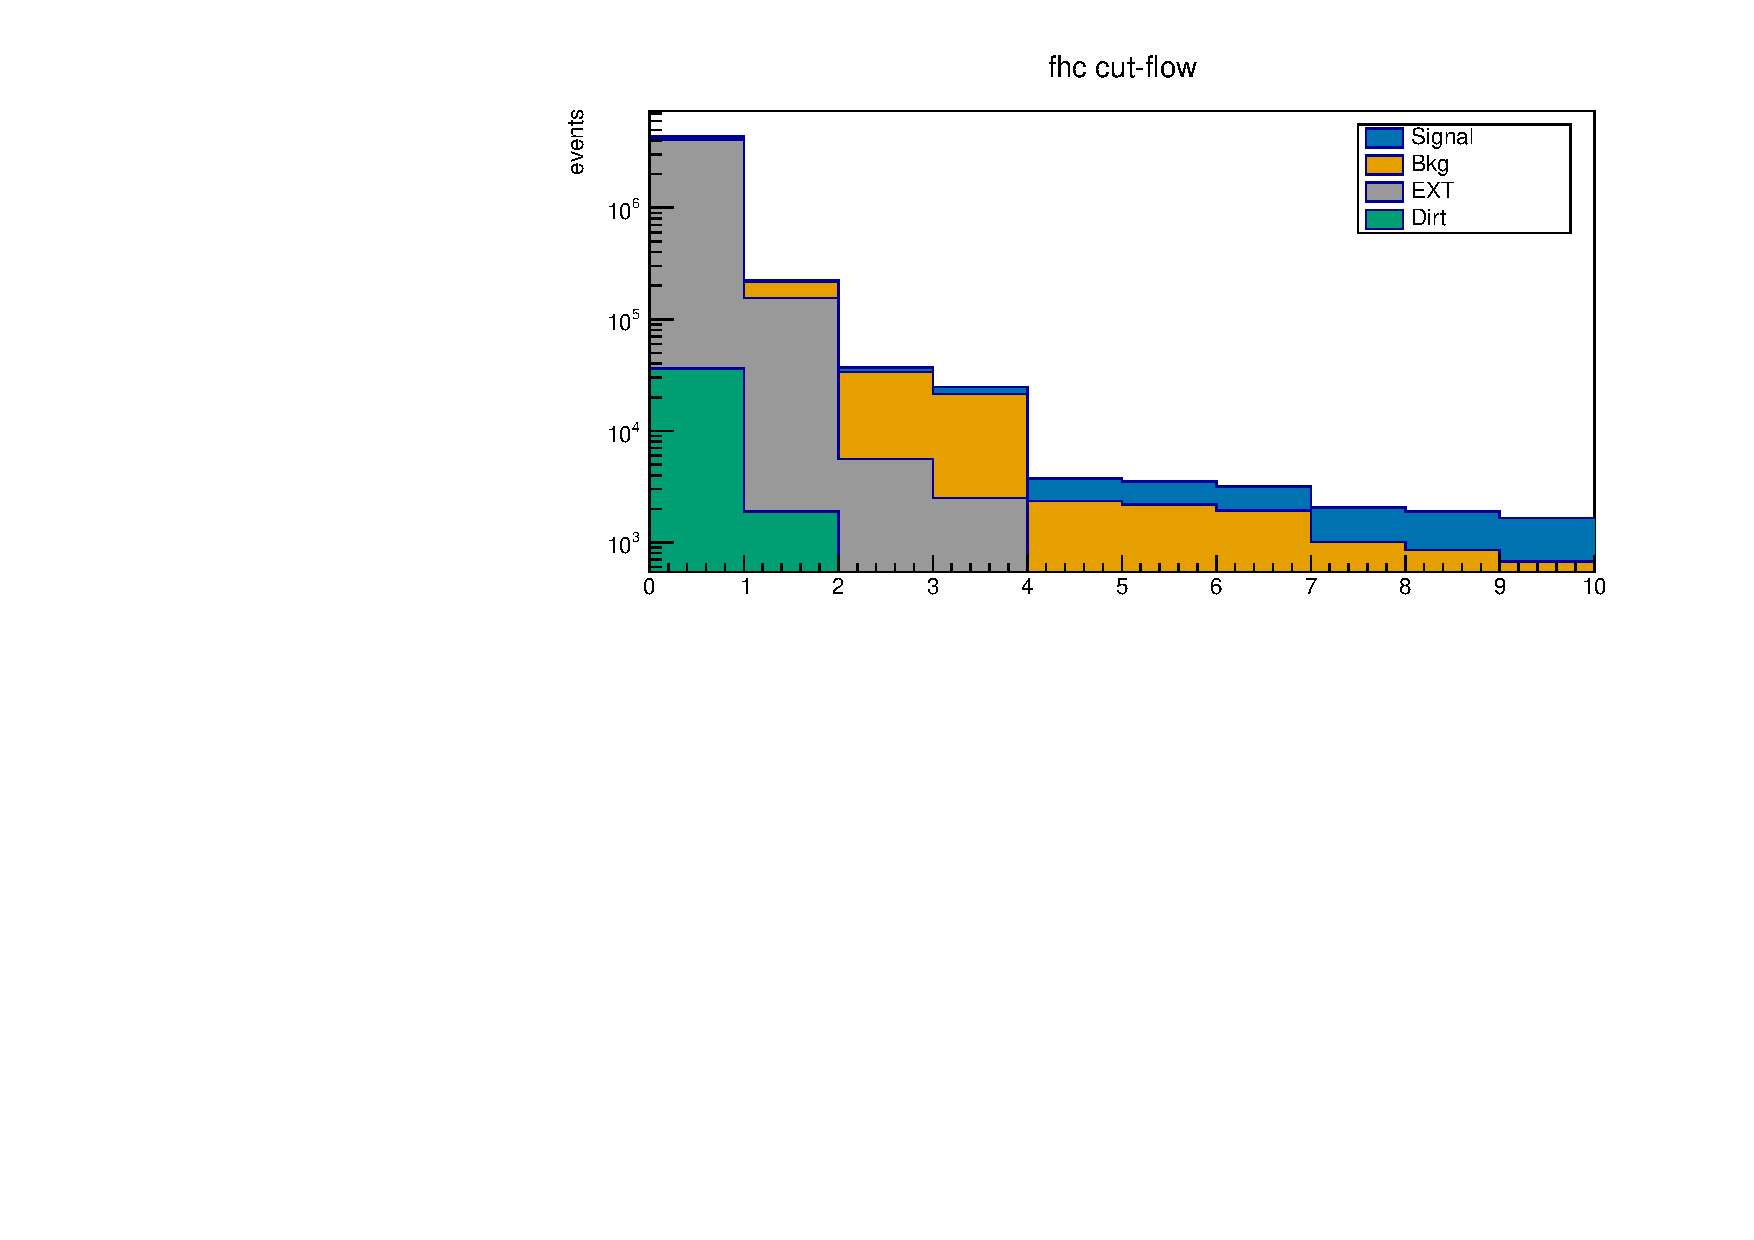
\includegraphics[width=\linewidth]{cutflow_yields_fhc}\\
  \centering{\scriptsize FHC cut-flow (signal blue, background orange, EXT grey, dirt green)}
  \end{columns}
\end{frame}

\begin{frame}{Reconstruction, response \& efficiency}
  \begin{columns}[c]
  \column{.34\textwidth}\centering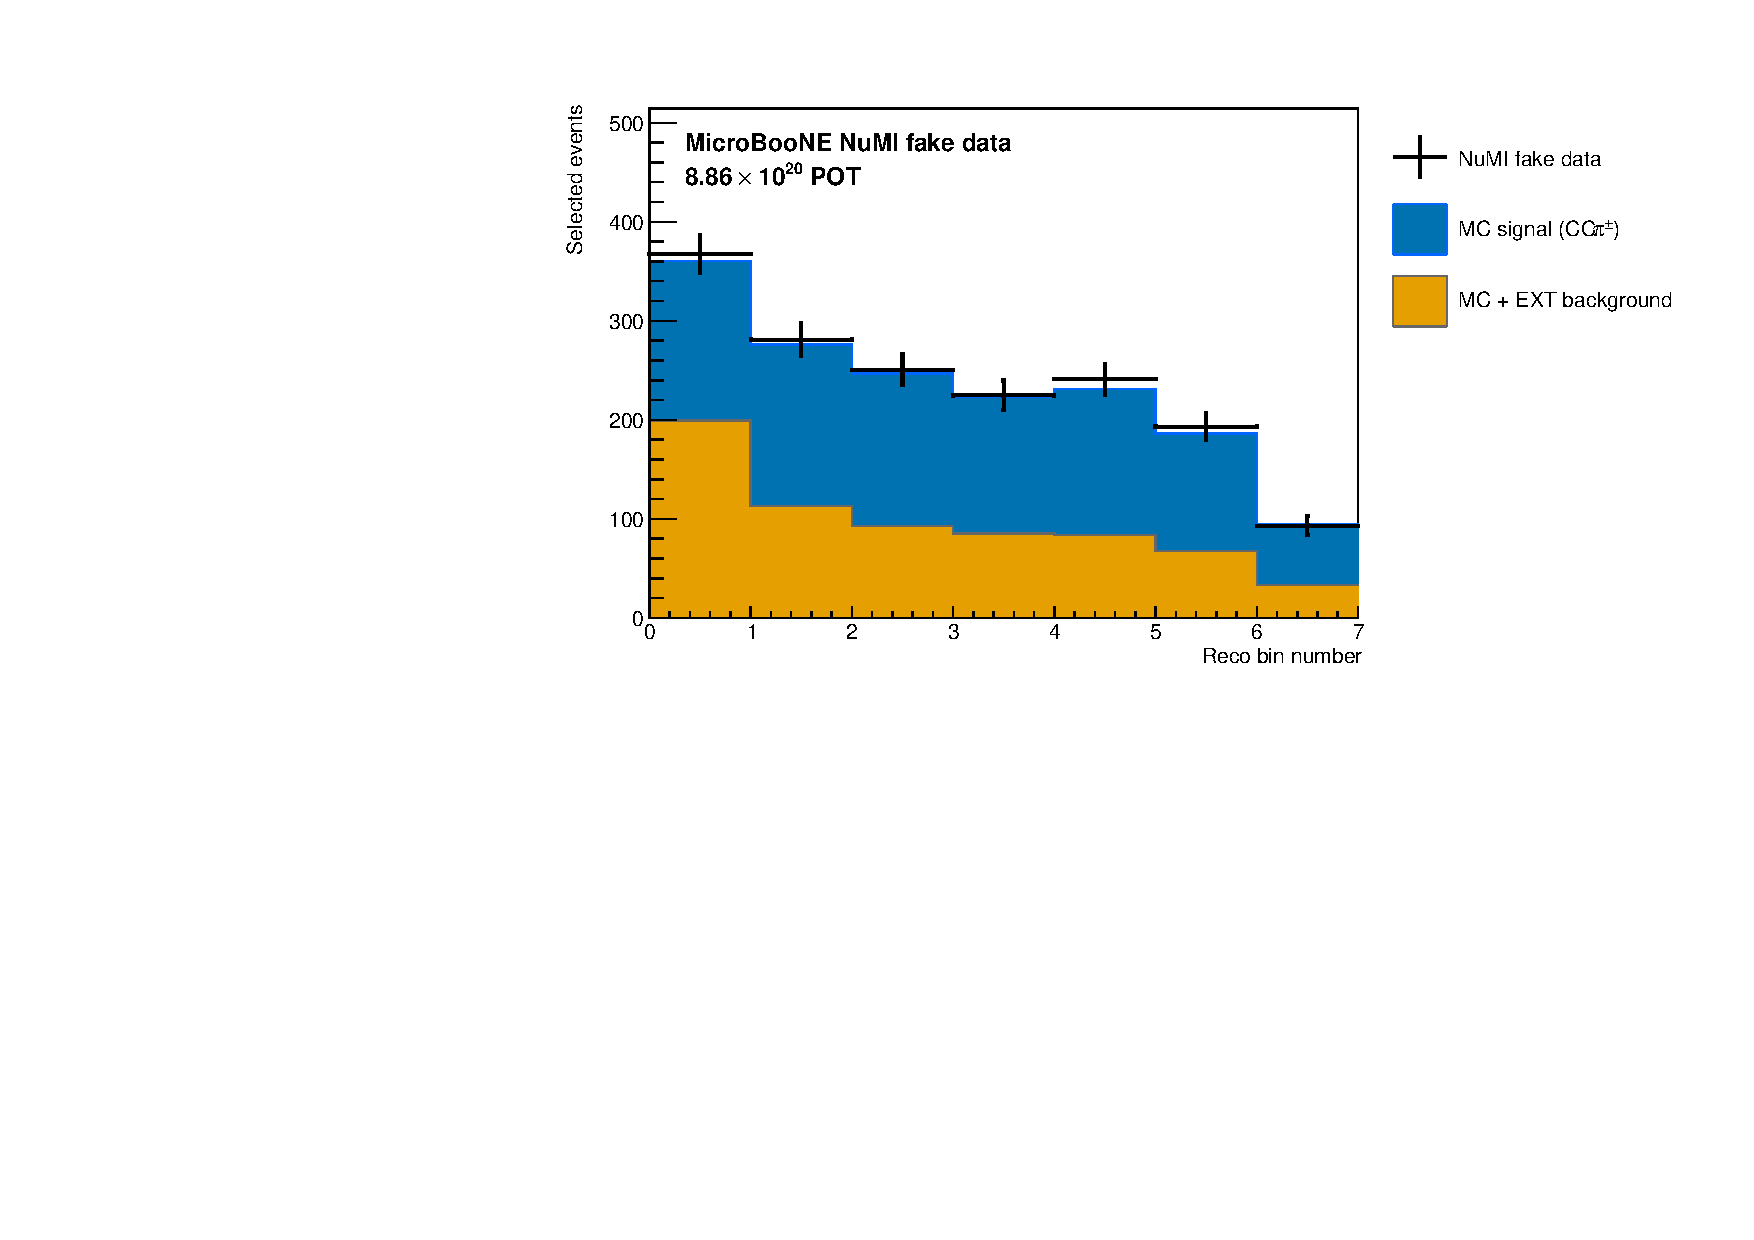
\includegraphics[width=\linewidth]{fw_reco_pmu}\\{\scriptsize Reco $p_\mu$ (data/MC stack)}
  \column{.33\textwidth}\centering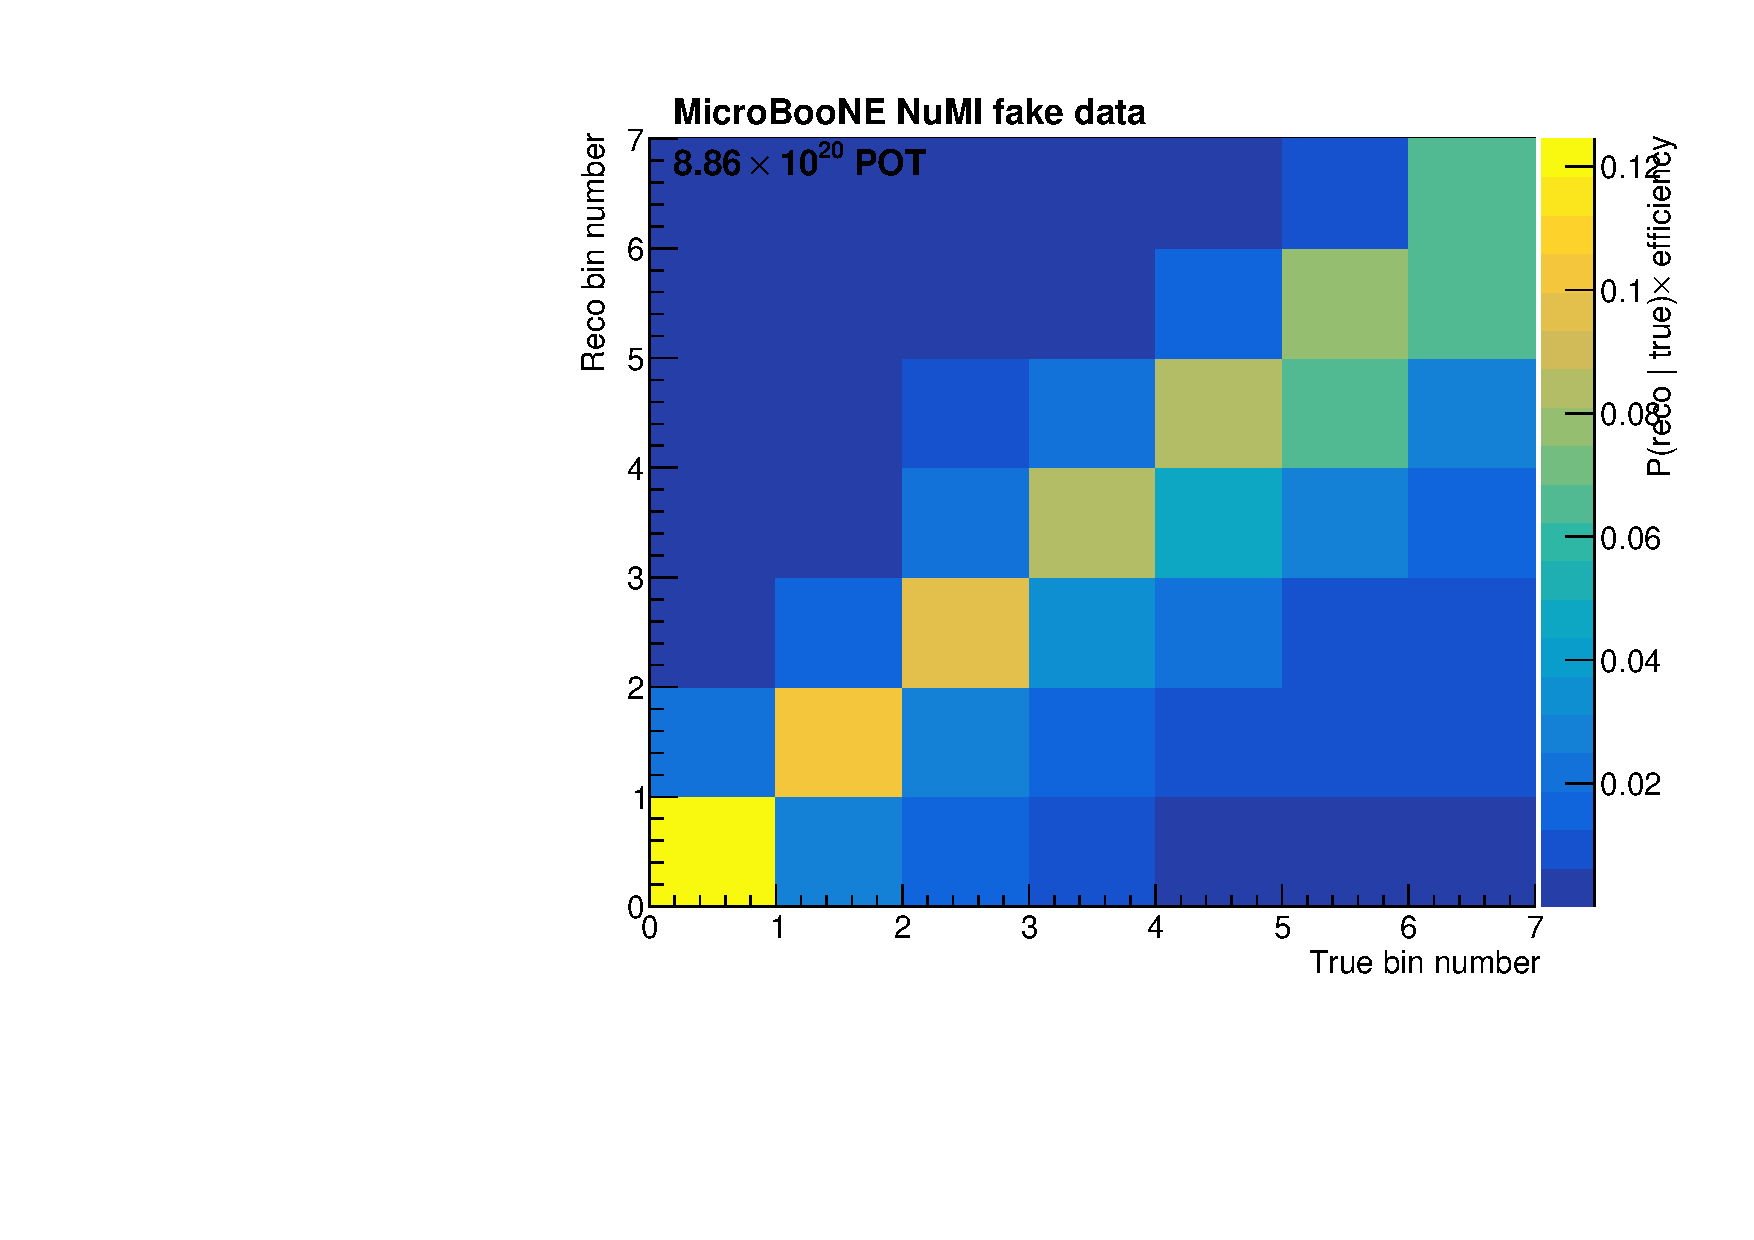
\includegraphics[width=\linewidth]{fw_resp_pmu}\\{\scriptsize Response matrix}
  \column{.33\textwidth}\centering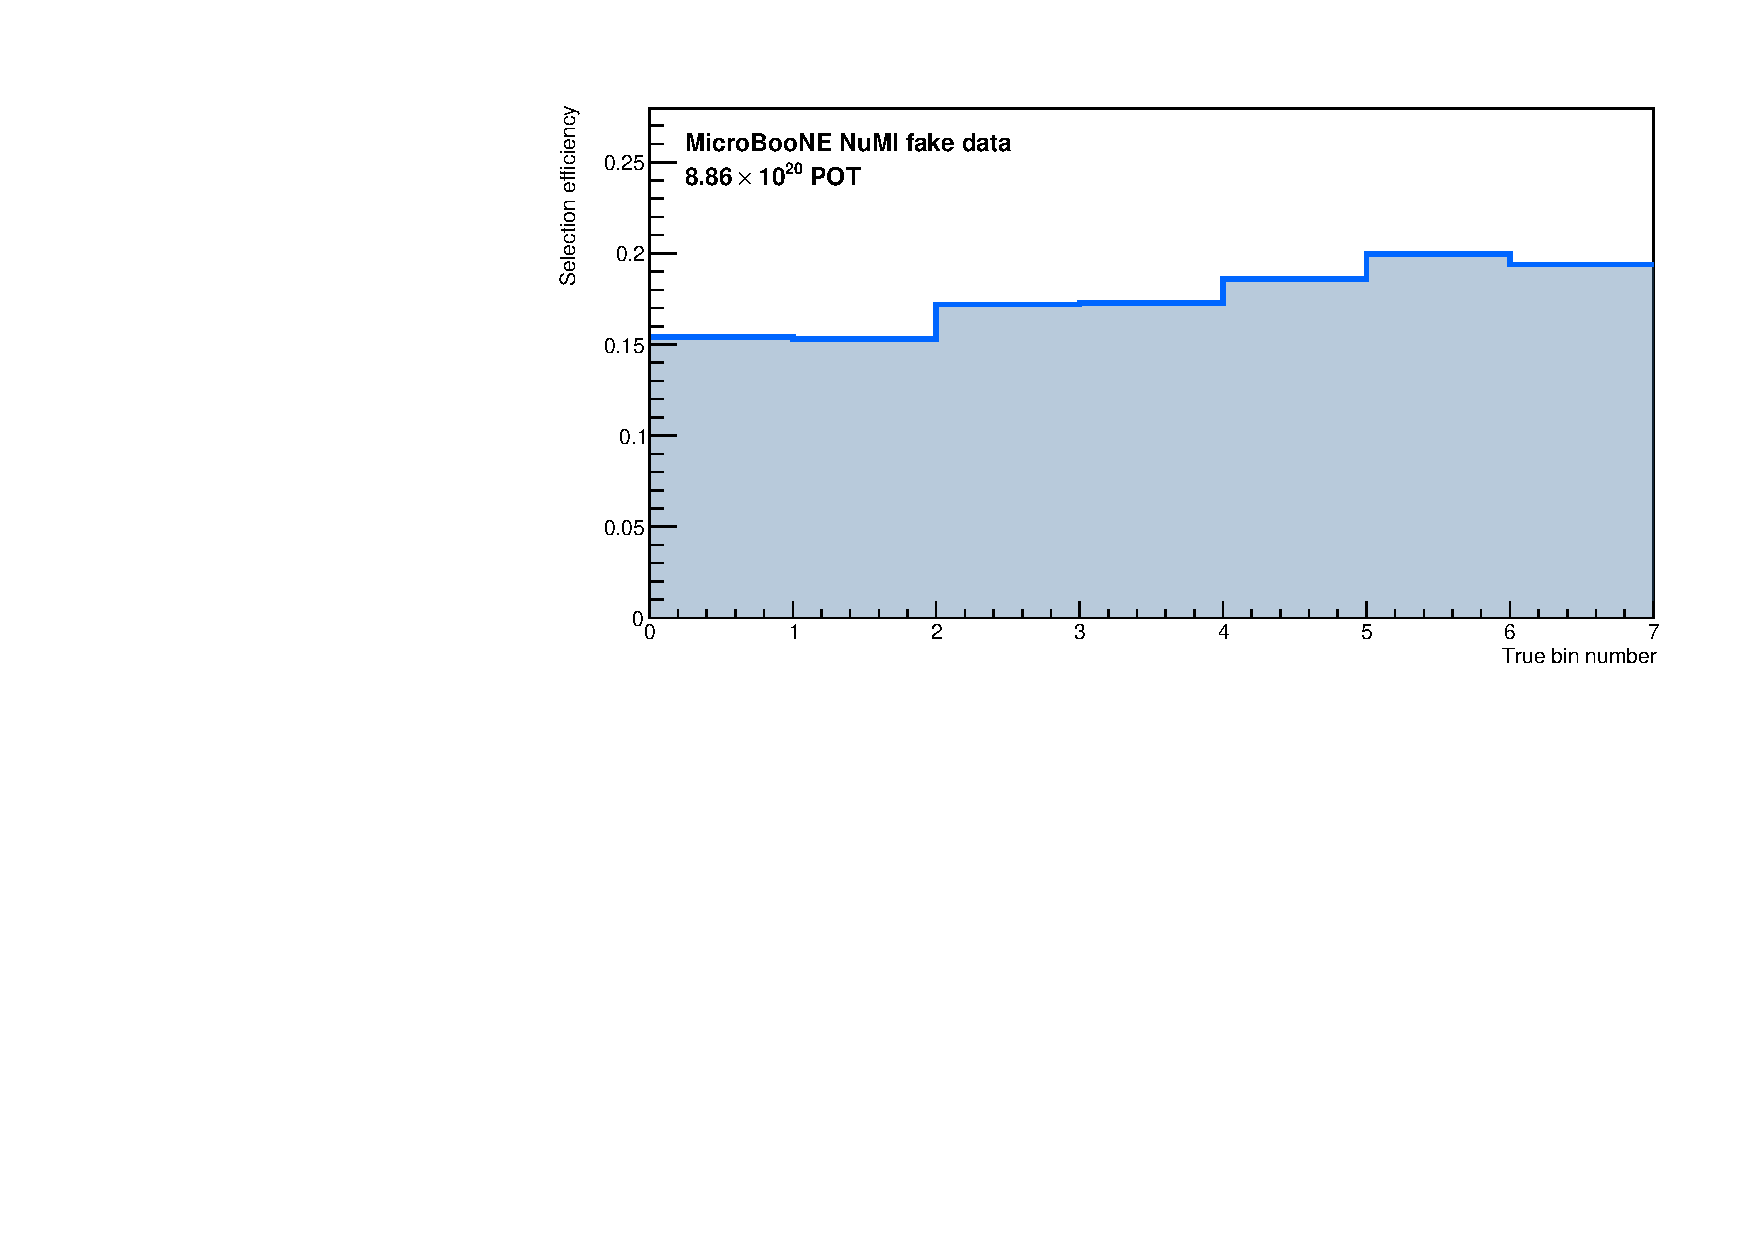
\includegraphics[width=\linewidth]{fw_eff_pmu}\\{\scriptsize Efficiency vs $p_\mu$}
  \end{columns}
  \vspace{1mm}
  \centering\small Wiener-SVD unfolding (framework \texttt{WienerSVDUnfolder}, 2nd-derivative
  regularisation) with the full systematic covariance from the universe throws.
\end{frame}

\begin{frame}{Differential cross sections --- FHC}
  \centering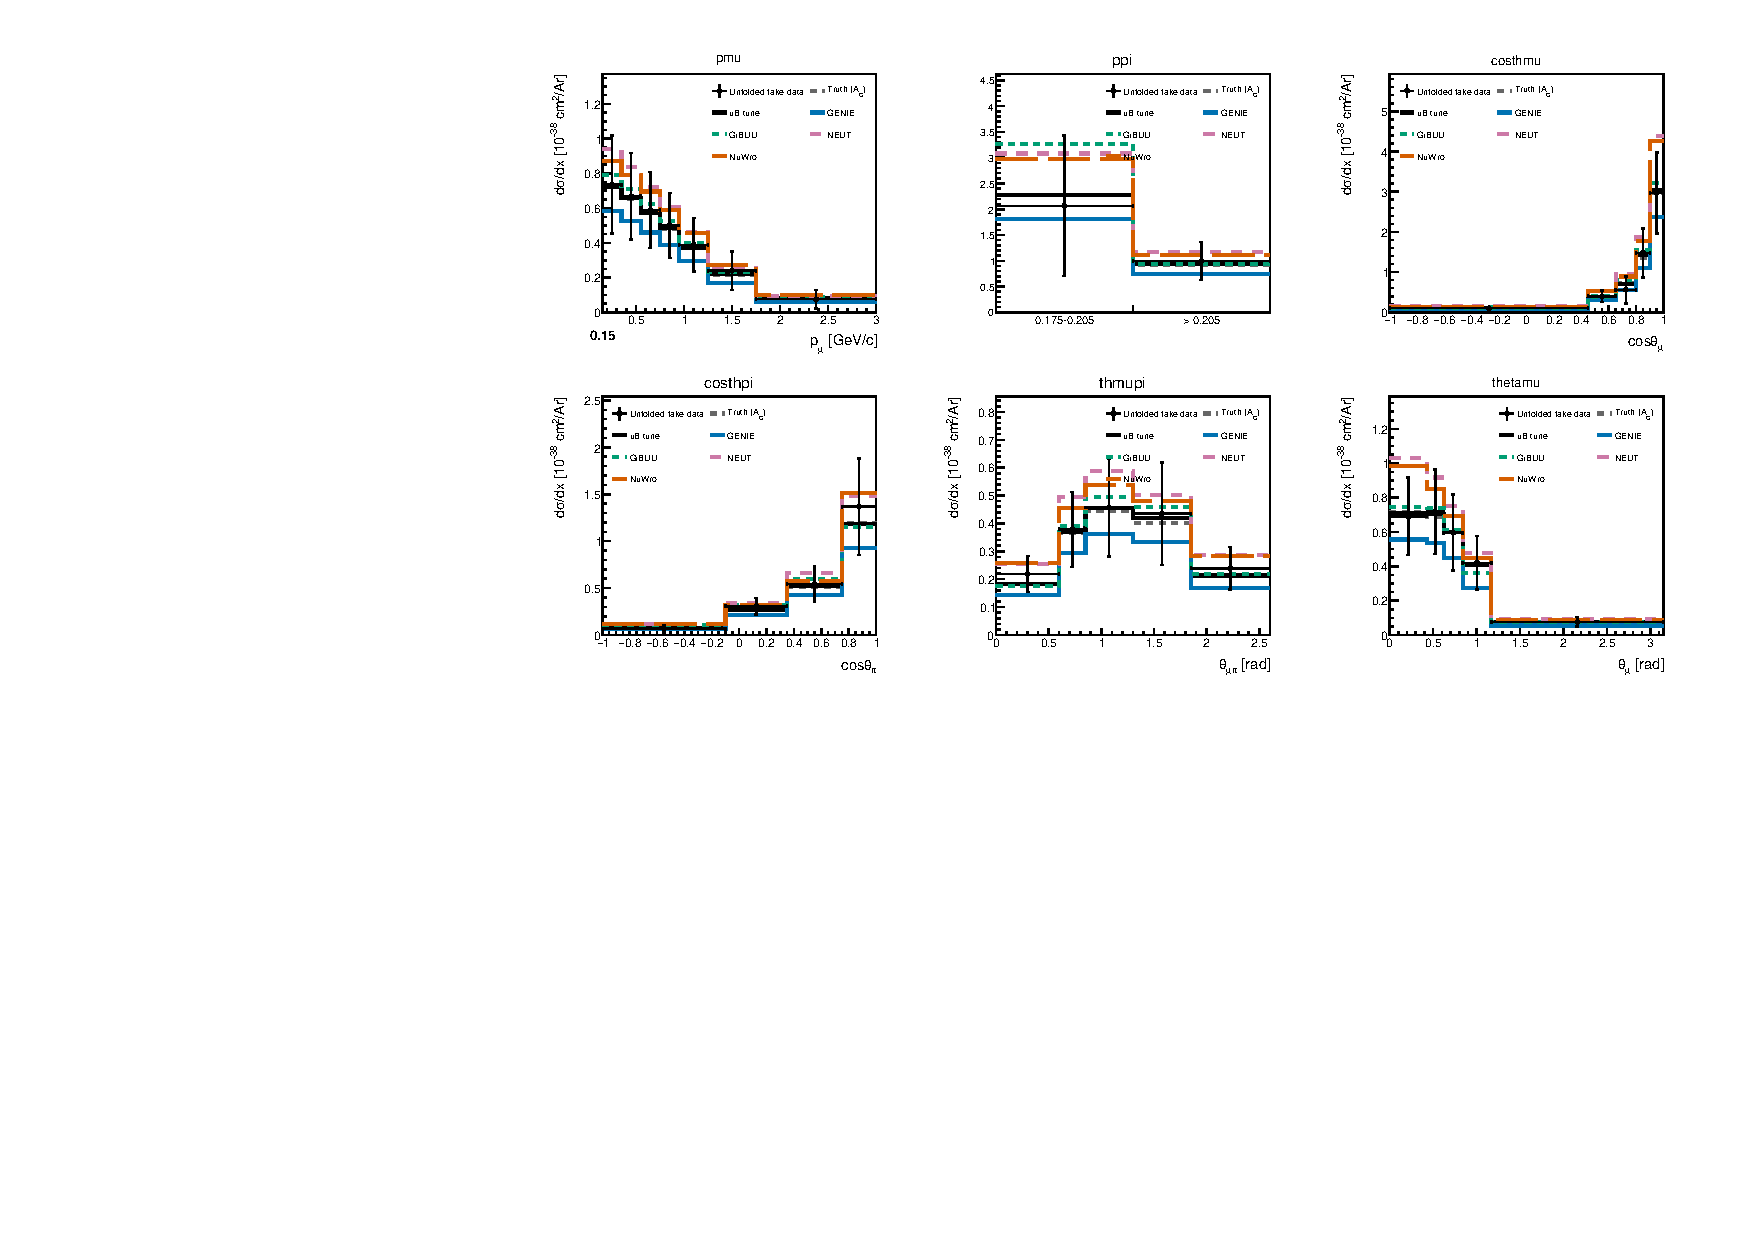
\includegraphics[height=.78\textheight]{dsigma_FHC5}\\
  {\scriptsize Unfolded fake data vs $A_C$-smeared truth, MicroBooNE tune, and GENIE/GiBUU/NEUT/NuWro.}
\end{frame}

\begin{frame}{Differential cross sections --- RHC}
  \centering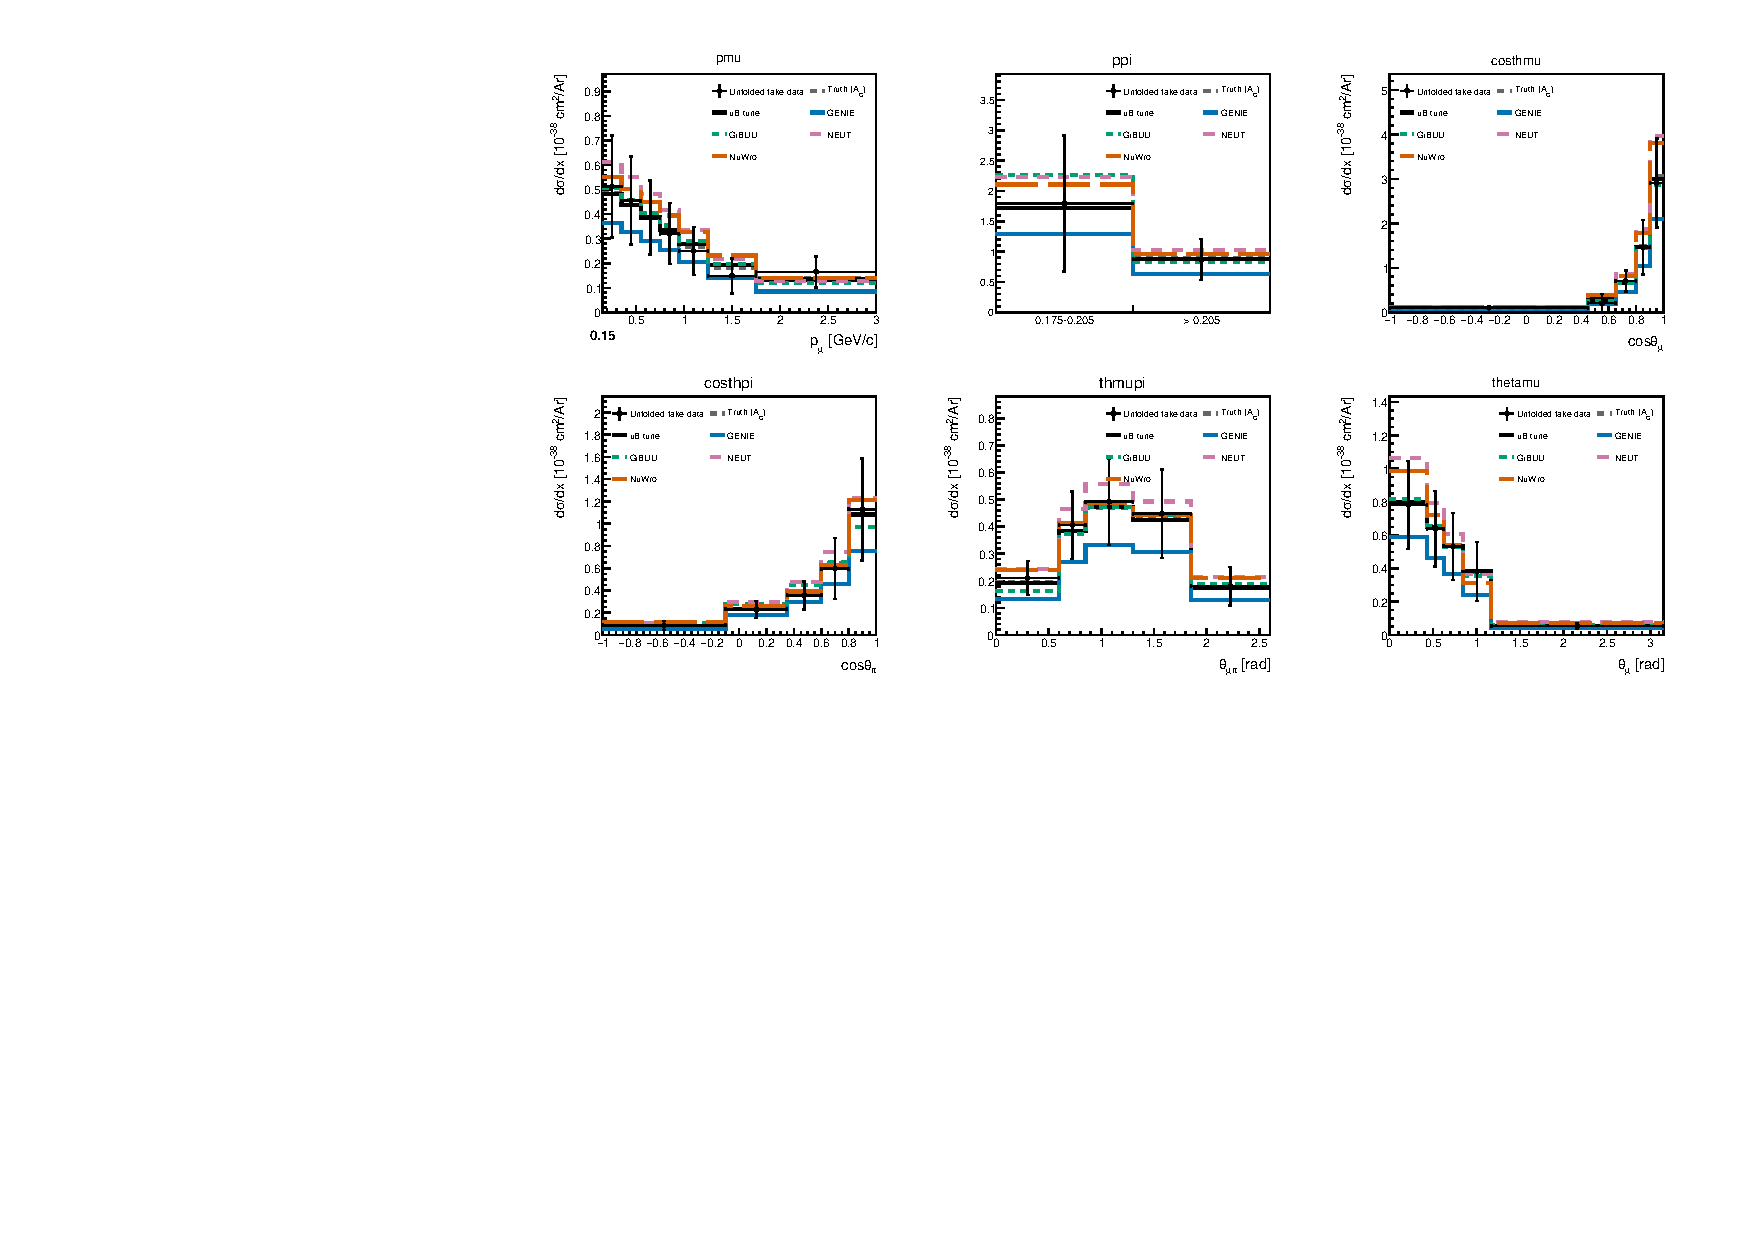
\includegraphics[height=.78\textheight]{dsigma_RHCFULL}\\
  {\scriptsize $\bar\nu_\mu$-enriched beam; unfolded fake data vs $A_C$-smeared truth,
  MicroBooNE tune, and GENIE/GiBUU/NEUT/NuWro.}
\end{frame}

\begin{frame}{Differential cross sections --- combined}
  \centering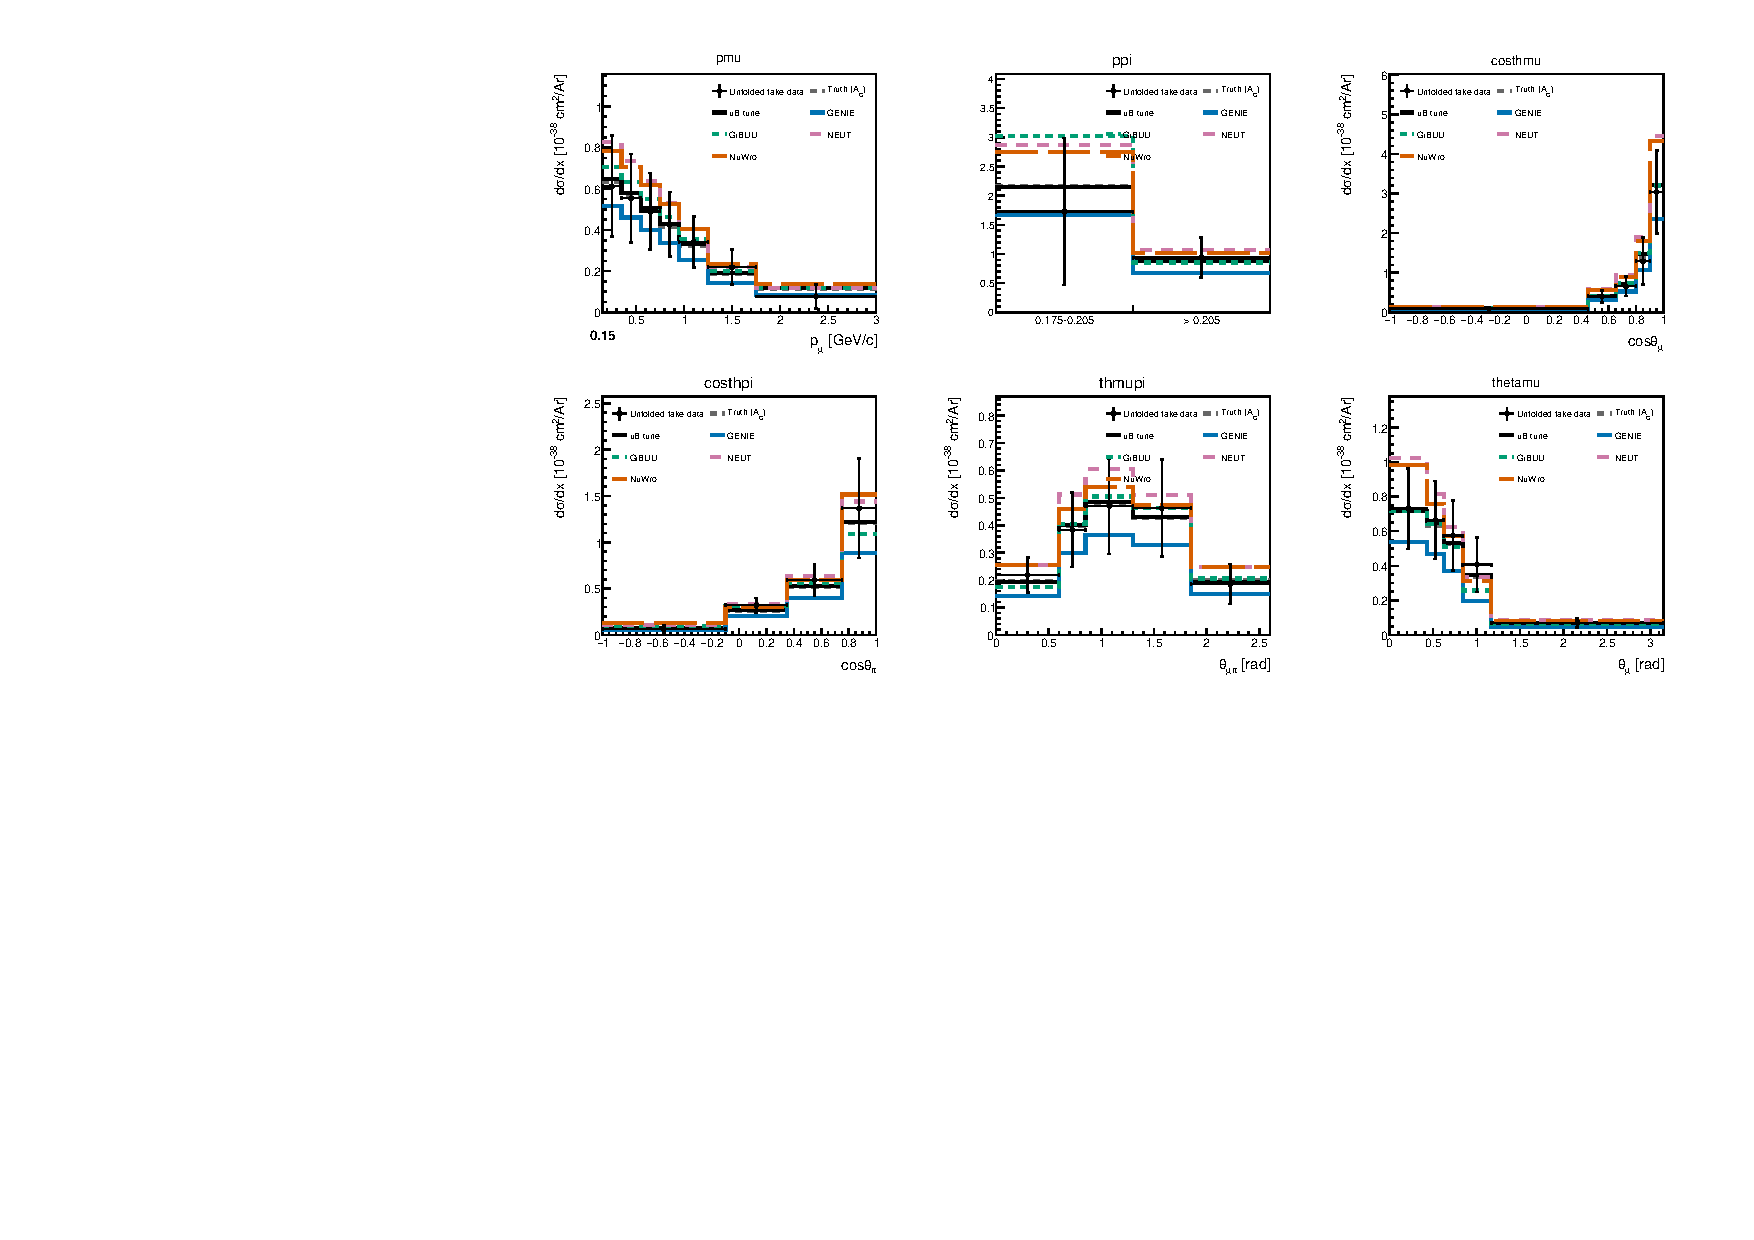
\includegraphics[height=.78\textheight]{dsigma_COMB}\\
  {\scriptsize FHC$+$RHC combined exposure (per-universe correlated flux treatment).}
\end{frame}

\begin{frame}{Integrated \& total flux-averaged cross section}
  \begin{columns}[T]\column{.5\textwidth}
  \begin{block}{Integrated $\sigma_\mathrm{int}$ (Wiener-SVD)}\footnotesize
  \begin{tabular}{lccc}
  \toprule & FHC & RHC & Comb\\\midrule
  $p_\mu$ & 0.99 & 1.02 & 0.88\\
  $p_\pi$ & 0.98 & 1.19 & 1.11\\
  $\cos\theta_\mu$ & 0.81 & 0.90 & 0.77\\
  $\cos\theta_\pi$ & 0.98 & 1.06 & 0.97\\
  $\theta_{\mu\pi}$ & 0.88 & 0.92 & 0.95\\
  \bottomrule
  \end{tabular}\\[1mm]
  {\scriptsize spread = Wiener-SVD $A_C$ smearing ($10^{-38}$cm$^2$/Ar)}
  \end{block}
  \column{.5\textwidth}
  \begin{block}{Total (cut-and-count, no unfolding)}\footnotesize
  \begin{tabular}{lc}
  \toprule Config & $\sigma$ ($10^{-38}$cm$^2$/Ar)\\\midrule
  FHC & $1.06\pm0.27$\\
  RHC & $0.98\pm0.35$\\
  Combined & $1.02\pm0.30$\\
  \bottomrule
  \end{tabular}\\[1mm]
  {\scriptsize FHC generators: GENIE 0.79, GiBUU 1.08, NEUT 1.26, NuWro 1.20 — agree within $\sim1\sigma$.}
  \end{block}
  \end{columns}
\end{frame}

\begin{frame}{Systematics \& sideband validation}
  \begin{columns}[T]\column{.55\textwidth}
  \centering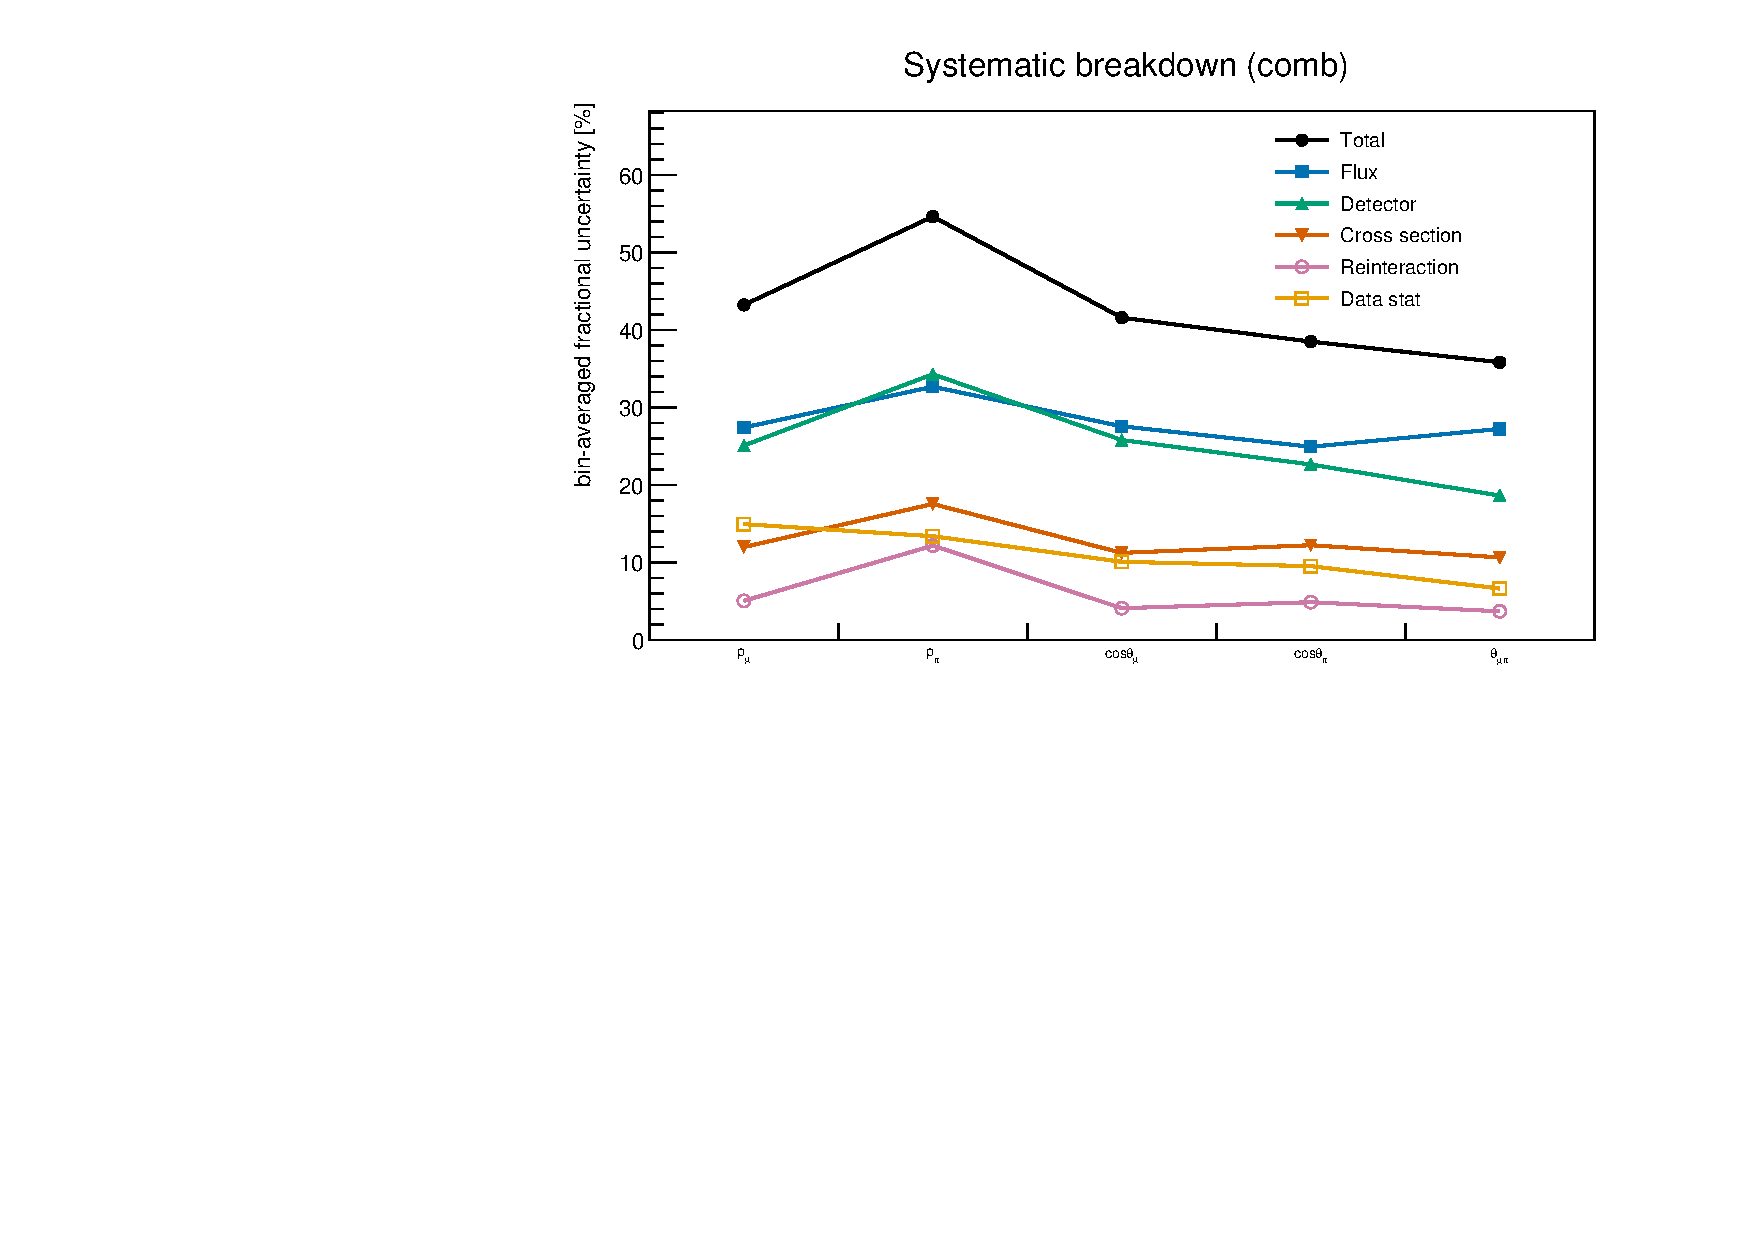
\includegraphics[width=\linewidth]{fw_systbreak_comb}\\
  {\scriptsize Flux (PPFX) dominates; detector second; total $\sim30$--$40\%$.}
  \column{.45\textwidth}
  \begin{block}{Background-control sidebands}\footnotesize
  Four signal-depleted regions (CC$0\pi$, multi-$\pi$, $\pi^0$, cosmic).
  High-statistics data$/\nu$MC $=1.00$ across FHC/RHC/comb $\Rightarrow$ per-run
  weighting \& POT machinery validated; ready to constrain the background at unblinding.
  \end{block}
  \end{columns}
\end{frame}

% ===================== PART II : PROTON-TAGGED =====================
\section{Proton-tagged}
\begin{frame}{Part II --- Proton-tagged subsample: hadronic mass \& TKI}
  \begin{block}{Idea}
    Requiring an identified proton reconstructs the full hadronic system, opening two
    new observable classes: the \alert{hadronic invariant mass} (probes
    $\Delta/N^\ast$ directly) and the \alert{transverse kinematic imbalance} (Fermi
    motion + FSI).
  \end{block}
  \begin{itemize}\small
    \item \texttt{CC1mu1pi1p}: inherits the inclusive selection + a leading proton
      (LLR PID, $p_p\ge0.3$~GeV/$c$, contained). Efficiency $11.5\%$, purity $48\%$.
    \item Six observables: $W_{\pi p}$, $W_\mathrm{had}$, $\delta p_T$,
      $\delta\alpha_T$, $\delta\phi_T$, $p_n$ (4 bins each).
  \end{itemize}
\end{frame}

\begin{frame}{Selection performance \& proton-tag quality}
  \begin{columns}[T]\column{.55\textwidth}
  \centering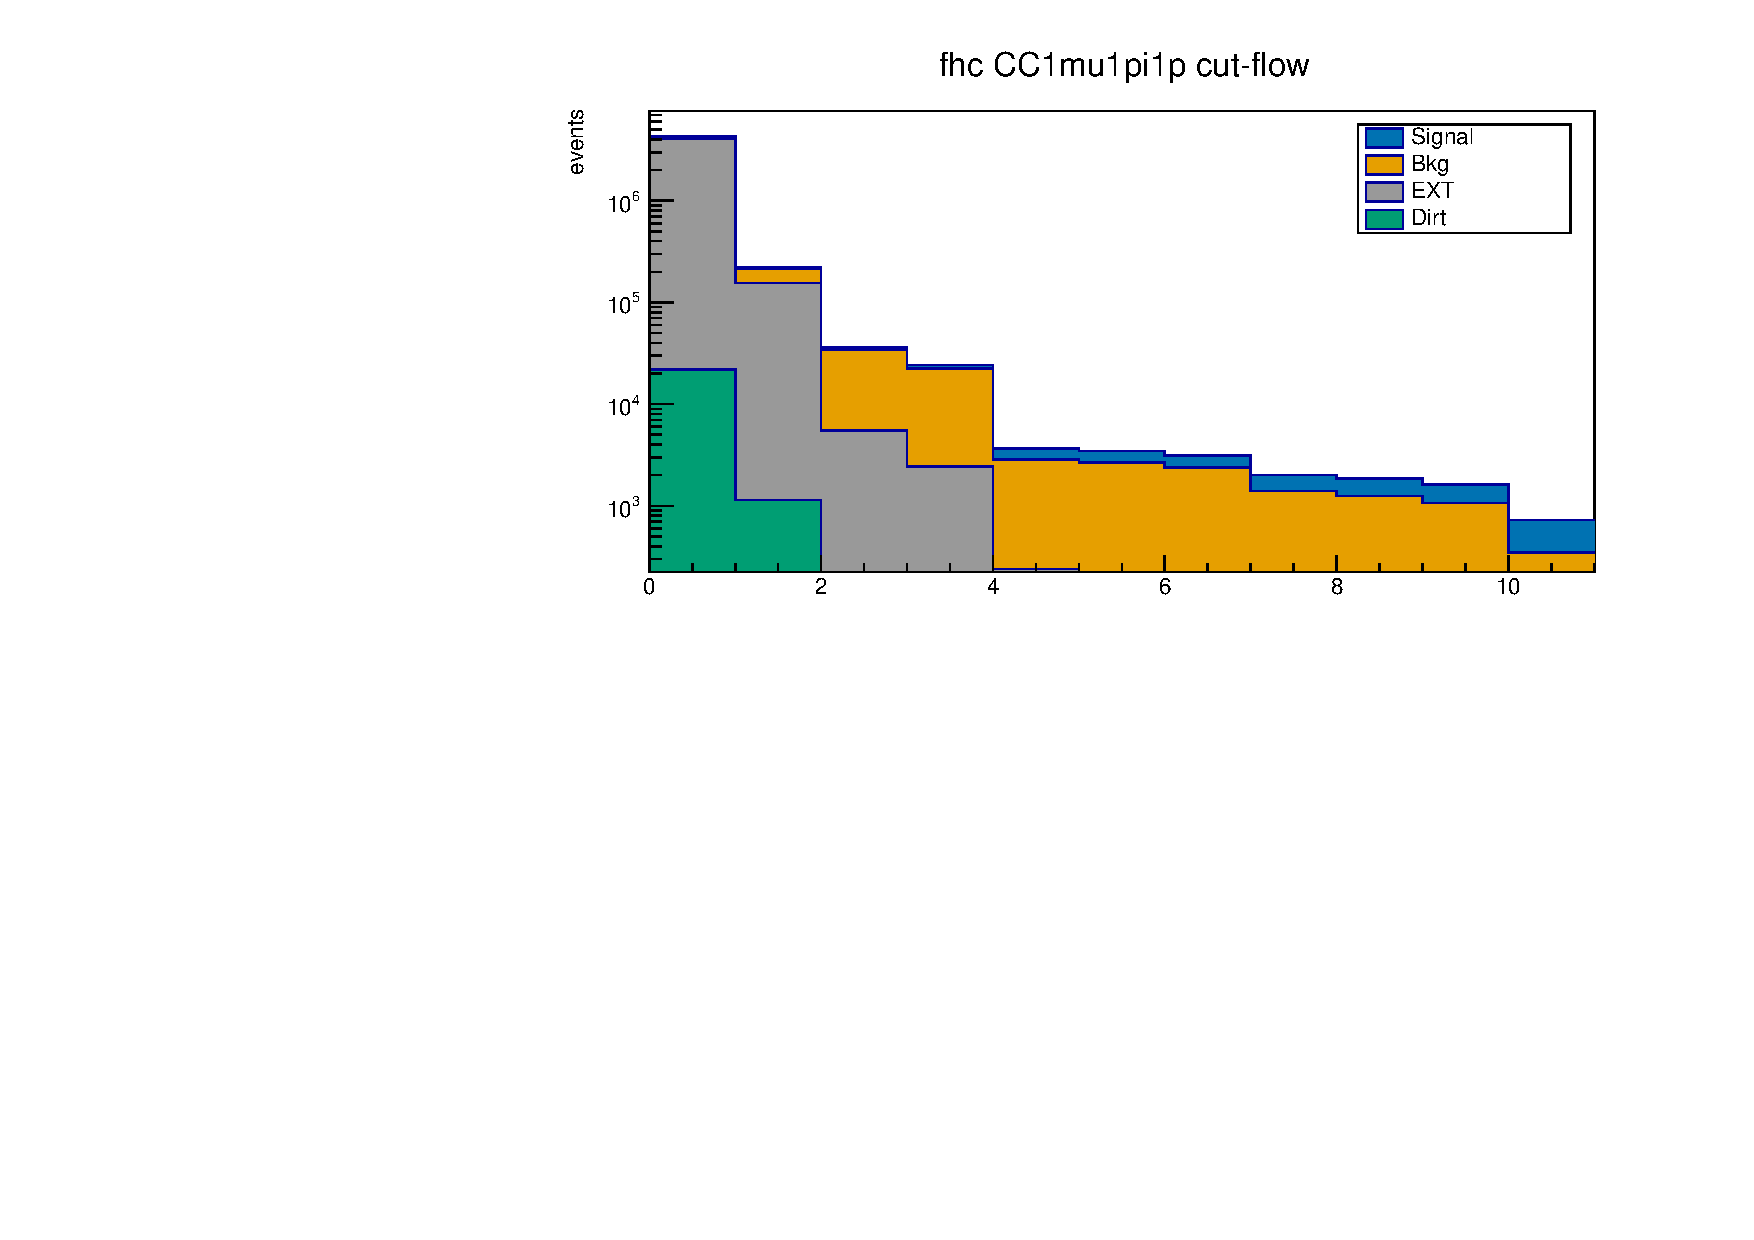
\includegraphics[width=\linewidth]{cutflow_yields_1p_fhc}\\
  {\scriptsize FHC proton-tagged cut-flow; last stage = proton identification}
  \column{.45\textwidth}
  \begin{block}{Proton tag (truth-matched, FHC)}\footnotesize
  \begin{itemize}
    \item $87\%$ tag purity ($\sim13\%$ mis-tag)
    \item Rejects $\sim64\%$ background for $\sim30\%$ signal loss
    \item Purity $33\%\to48\%$; $S/\sqrt{B}$ $+17\%$
    \item Proton $p$: $-9\%$ bias, $21\%$ resolution
  \end{itemize}
  \end{block}
  \end{columns}
\end{frame}

\begin{frame}{Proton-tagged differential cross sections (FHC)}
  \centering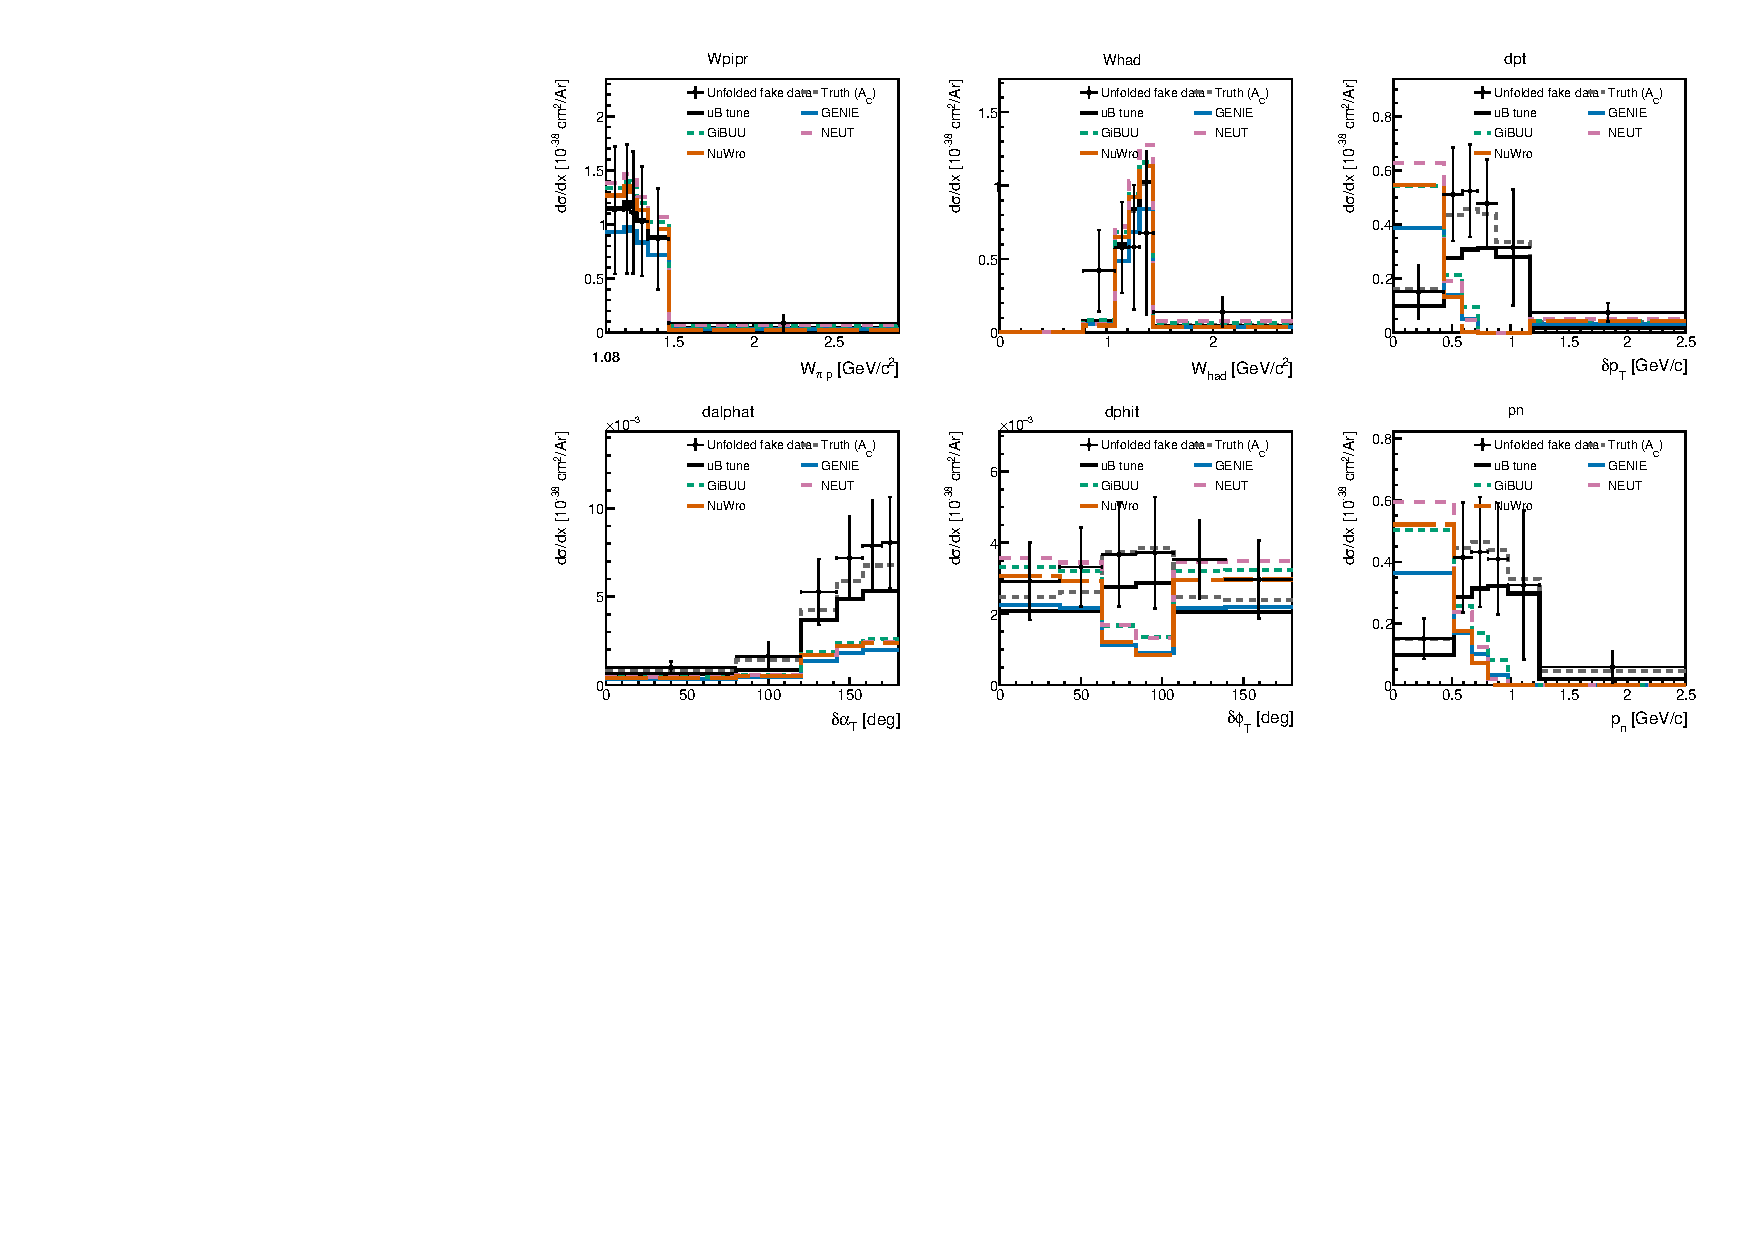
\includegraphics[height=.72\textheight]{dsigma_ccpi1p_FHC5}\\
  {\scriptsize Unfolded fake data vs truth, uB tune, and all four generators.
  Closure $\chi^2/\mathrm{ndf}\ll1$ for every observable.}
\end{frame}

\begin{frame}{Generator comparison \& background composition}
  \begin{columns}[T]\column{.5\textwidth}
  \begin{block}{Integrated proton-tagged $\sigma$ ($10^{-38}$cm$^2$/Ar)}\footnotesize
  GENIE 0.50 $<$ NuWro 0.65 $<$ GiBUU 0.74 $<$ NEUT 0.78; data $\sim0.58$.\\
  Spread $\sim1.6\times$; largest in low-$\delta p_T$/high-$p_n$ (FSI-sensitive).\\[1mm]
  {\scriptsize NuWro/NEUT reprocessed from event vectors in the SL7 container.}
  \end{block}
  \column{.5\textwidth}
  \begin{block}{Remaining background (FHC)}\footnotesize
  \begin{tabular}{lr}
  \toprule Component & \%\\\midrule
  $\nu_\mu$ CC wrong topology & 64\\
  True CC$1\mu1\pi$, no $p{>}0.3$ & 18\\
  NC & 11\\
  Out-of-FV & 5\\
  $\nu_e$ CC & 1\\
  \bottomrule
  \end{tabular}\\[1mm]
  {\scriptsize $82\%$ true $\nu_\mu$ CC — well modelled \& constrainable.}
  \end{block}
  \end{columns}
\end{frame}

\begin{frame}{Summary}
  \begin{itemize}
    \item \alert{Inclusive}: differential CC$1\mu1\pi^{\pm}$ cross sections for FHC, RHC
      and combined, per-run POT scaling, Wiener-SVD unfolding; total flux-averaged
      $\sigma$ agrees with GENIE/GiBUU/NEUT/NuWro within $\sim1\sigma$.
    \item \alert{Proton-tagged}: new hadronic-mass ($W_{\pi p}$, $W_\mathrm{had}$) and
      TKI ($\delta p_T$, $\delta\alpha_T$, $\delta\phi_T$, $p_n$) observables; FHC closure
      validated; all four generators compared and bracket the data.
    \item Blind analysis: fake data throughout; sidebands ready to constrain the
      background before unblinding.
    \item \alert{Ongoing}: RHC/combined W/TKI in production; detector systematic and a
      tighter-proton-PID study underway.
  \end{itemize}
  \vspace{2mm}
  \centering\color{ubred}\large Thank you --- questions?
\end{frame}

% ===================== BACKUP =====================
\appendix
\section{Backup}
{\setbeamercolor{frametitle}{fg=white,bg=ubdark}
\begin{frame}[plain]\centering\vfill
  {\color{ubdark}\Huge\bfseries Backup}\vfill
\end{frame}

\begin{frame}{Backup: per-run exposure}
  \centering\footnotesize
  \begin{tabular}{llrr}
  \toprule Mode & Run & Data POT & MC/data scale\\\midrule
  FHC & 1 & $3.28\times10^{20}$ & 0.141\\
      & 2 & $1.27\times10^{20}$ & 0.051\\
      & 4 & $2.08\times10^{20}$ & 0.073\\
      & 5 & $2.23\times10^{20}$ & 0.116\\
  RHC & 1--4 & $1.11\times10^{21}$ & 0.045--0.091\\
  \bottomrule
  \end{tabular}\\[2mm]
  {\scriptsize Each run scaled by its own $D_\mathrm{run}/\mathrm{MC}_\mathrm{run}$ (real-data-ready).}
\end{frame}

\begin{frame}{Backup: systematic breakdown (combined)}
  \centering\scriptsize
  \begin{tabular}{lccccc}
  \toprule Source & $p_\mu$ & $p_\pi$ & $\cos\theta_\mu$ & $\cos\theta_\pi$ & $\theta_{\mu\pi}$\\\midrule
  \textbf{Total} & 30.1 & 33.7 & 41.0 & 34.8 & 29.3\\
  Flux (PPFX) & 22.1 & 24.2 & 29.1 & 25.3 & 21.6\\
  Detector & 13.5 & 19.6 & 23.5 & 20.6 & 15.6\\
  Cross section & 9.4 & 8.5 & 9.9 & 8.6 & 7.6\\
  Data stat & 10.0 & 6.1 & 11.0 & 5.4 & 7.6\\
  \bottomrule
  \end{tabular}\\[2mm]
  {\scriptsize Bin-averaged fractional uncertainty [\%]. Flux dominates throughout.}
\end{frame}

\begin{frame}{Backup: W/TKI observable definitions}
  \small From the muon, charged-pion and leading-proton momenta (STV tool, option 1):
  \begin{align*}
  W_{\pi p} &= \sqrt{(E_\pi+E_p)^2-|\vec p_\pi+\vec p_p|^2}\quad\text{(direct, no $\nu$ direction)}\\
  W_\mathrm{had} &= \sqrt{m_p^2+2m_p(E_\mathrm{cal}-E_\mu)-Q^2}\quad\text{(calorimetric)}\\
  \delta p_T &= |\vec p_T^{\,\mu}+\vec p_T^{\,\mathrm{had}}|,\quad
  \delta\alpha_T,\ \delta\phi_T\ \text{(TKI angles)},\quad p_n=\sqrt{\delta p_T^2+p_L^2}
  \end{align*}
  Proton momentum from the proton-hypothesis range kinetic energy;
  $E_b=24.78$~MeV argon removal energy.
\end{frame}

\begin{frame}{Backup: proton-tagged binning \& closure}
  \centering\footnotesize
  \begin{tabular}{ll}
  \toprule Observable & Bin edges\\\midrule
  $W_{\pi p}$ & 1.08, 1.20, 1.32, 1.50, 2.00 GeV/$c^2$\\
  $W_\mathrm{had}$ & 0, 1.00, 1.20, 1.40, 1.90 GeV/$c^2$\\
  $\delta p_T$ & 0, 0.45, 0.70, 1.00, 1.60 GeV/$c$\\
  $\delta\alpha_T$ & 0, 90, 130, 160, 180 deg\\
  $\delta\phi_T$ & 0, 50, 85, 125, 180 deg\\
  $p_n$ & 0, 0.55, 0.80, 1.10, 1.70 GeV/$c$\\
  \bottomrule
  \end{tabular}\\[2mm]
  {\scriptsize FHC closure $\sigma_\mathrm{int}$: 0.64, 0.59, 0.56, 0.56, 0.63, 0.54;
  $\chi^2/\mathrm{ndf}=1.5,0.2,0.4,0.5,0.3,0.1$ over 4 bins.}
\end{frame}

\begin{frame}{Backup: generator predictions}
  \small
  \begin{itemize}
    \item Inclusive: per-observable $d\sigma/dx$ from GENIE (gst), GiBUU
      (\texttt{FinalEvents}), NEUT (neutvect), NuWro (event output), flux-combined to
      per-argon $10^{-38}$~cm$^2$.
    \item Proton-tagged W/TKI: same event samples reprocessed with the proton tag +
      TKI construction; NuWro and NEUT run inside the SL7 apptainer container.
    \item FTE rebinned to the coarsened analysis binning so every generator overlays
      on every observable.
  \end{itemize}
\end{frame}
}

\end{document}
